\documentclass[12pt]{article}
\usepackage[utf8]{inputenc}
\usepackage[T1]{fontenc} % uses T1 fonts (better quality)
\usepackage{lmodern} % uses Times fonts
% \usepackage{mathptmx} % uses Times fonts
\usepackage[dvipsnames]{xcolor}
\usepackage[margin=1in]{geometry}
\usepackage{nopageno} % no page numbers
\usepackage{graphicx}
\usepackage{bm}
\graphicspath{ {./img/} }
\usepackage{booktabs}   % for table borders
\usepackage{colortbl}
\usepackage{float}

\title{ECE440-HW05}
\begin{document}
% \begin{titlepage}
% \vspace*{\fill}
 	\begin{center}
     \line(1,0){300}\\[0.25cm]
 	\Large{\bfseries ECE440: Homework \#5}\\
 	\textsc{\large David Kirby}\\
 	\textsc{\large Due: 07 May 2020}\\
 	\line(1,0){300}\\[0.75cm]
 	\end{center}
 %	\vfill
% \end{titlepage}
 
\begin{enumerate}
\bfseries \item Problem P3, Chapter 5 (50\%)\\[1em]
Consider the following network. With the indicated link costs, use Dijkstra’s shortest-path algorithm to compute the shortest path from $\bm{x}$ to all nodes. Show how the algorithm works by computing a table similar to Table 5.1.\par
\begin{figure}[h!]
    \centering
    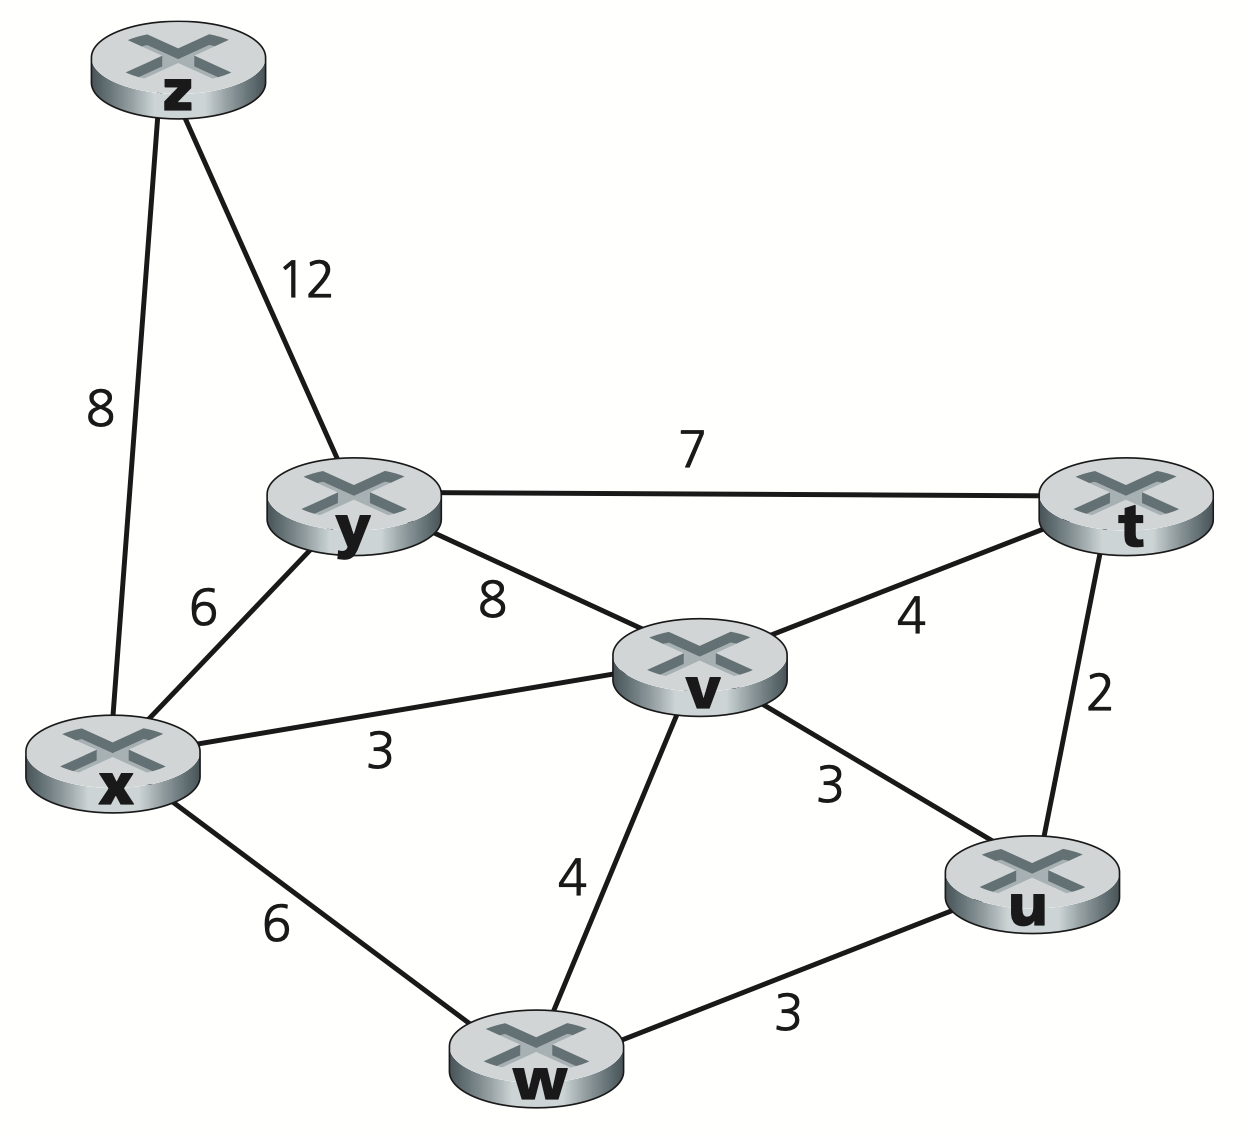
\includegraphics[width=0.35\textwidth]{Screen Shot 2020-05-04 at 23.25.42.png}
    % \caption{}
    % \label{fig:I2Cdemo}
\end{figure}
\begin{table}[ht]
\centering
\begin{tabular}{@{}lccccccc@{}}
\arrayrulecolor{RoyalBlue}\toprule
Step & N'      & D(z),p(z)                  & D(y),p(y)                  & D(w),p(w)                  & D(v),p(v)                  & D(u),p(u)                  & D(t),p(t)                  \\ \midrule
0    & x       & 8,x                        & 6,x                        & 6,x                        & {\color[HTML]{FE0000} 3,x} & $\infty$                      & $\infty$                      \\
1    & vx      & 8,x                        & 6,x                        & {\color[HTML]{FE0000} 6,x} & -                          & 6,v                        & 7,v                        \\
2    & vwx     & 8,x                        & {\color[HTML]{FE0000} 6,x} & -                          & -                          & 6,v                        & 7,v                        \\
3    & vwxy    & 8,x                        & -                          & -                          & -                          & {\color[HTML]{FE0000} 6,v} & 7,v                        \\
4    & uvwxy   & 8,x                        & -                          & -                          & -                          & -                          & {\color[HTML]{FE0000} 7,v} \\
5    & tuvwxy  & {\color[HTML]{FE0000} 8,x} & -                          & -                          & -                          & -                          & -                          \\
6    & tuvwxyz & -                          & -                          & -                          & -                          & -                          & -                          \\ \bottomrule
\end{tabular}
\end{table}
\newpage
\bfseries \item Problem P5, Chapter 5 (50\%)\\[1em]
Consider the network shown below, and assume that each node initially knows the costs to each of its neighbors. Consider the distance-vector algorithm and show the distance table entries at node $\bm{z}$.\par
\begin{figure}[h!]
    \centering
    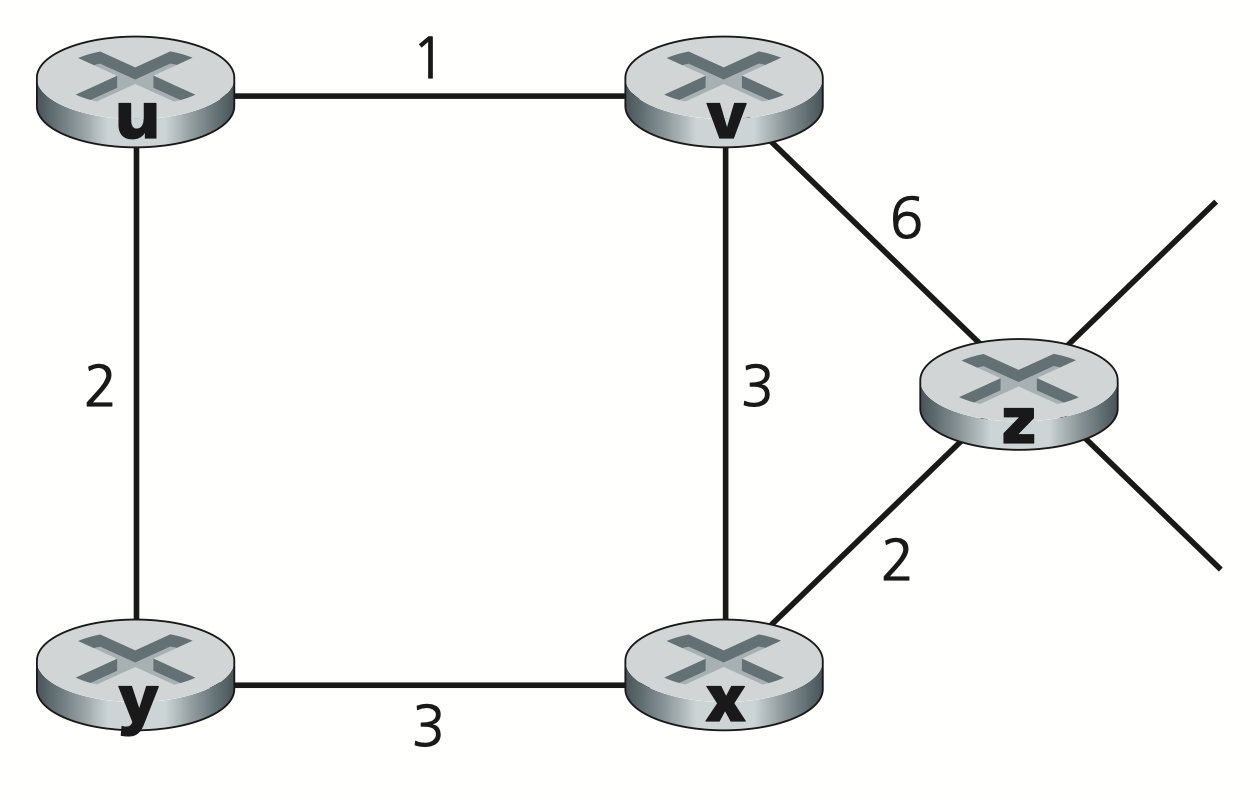
\includegraphics[width=0.35\textwidth]{Screen Shot 2020-05-05 at 00.33.53.png}
    % \caption{}
    % \label{fig:I2Cdemo}
\end{figure}
% Please add the following required packages to your document preamble:
% \usepackage{booktabs}
\begin{table}[ht]
\centering
\caption{Initial Neighbors\hspace{4.5em}Table 2: After One-hop}\vspace{1em}
\begin{tabular}{cc|ccccc ccc c|cccccc ccc c|cccccc}
        &       &           &           &to         &           &           &&&         &       &           &           &to         &           &               \\
        &       & u         & v         & x         & y         & z         &&&         &       & u         & v         & x         & y         & z             \\ \cline{2-7}\cline{11-16}
        & u     & $\infty$  & $\infty$  & $\infty$  & $\infty$  & $\infty$  &&&         & u     & 0         & 1         & $\infty$  & 2         & $\infty$      \\
        & v     & $\infty$  & $\infty$  & $\infty$  & $\infty$  & $\infty$  &&&         & v     & 1         & 0         & 3         & $\infty$  & 6             \\
\rotatebox[origin=c]{90}{from}    & x     & $\infty$  & $\infty$  & $\infty$  & $\infty$  & $\infty$  &&& \rotatebox[origin=c]{90}{from}    & x     & $\infty$  & 3         & 0         & 3         & 2             \\
        & y     & $\infty$  & $\infty$  & $\infty$  & $\infty$  & $\infty$  &&&         & y     & 2         & $\infty$  & 3         & 0         & $\infty$      \\
        & z     & $\infty$  & 6         & 2         & $\infty$  & $\infty$  &&&         & z     & $\infty$  & 6         & 2         & $\infty$  & 0
\end{tabular}
\end{table}\par
\setcounter{table}{+2}
\begin{table}[ht]
\centering
\caption{Minimum distance vectors}\vspace{1em}

\begin{tabular}{cc|ccccc}
        &       &           &           &to         &           &           \\
        &       & u         & v         & x         & y         & z         \\ \cline{2-7}
        & u     & 0         & 1         & 4         & 2         & 6         \\
        & v     & 1         & 0         & 3         & 3         & 5         \\
\rotatebox[origin=c]{90}{from}    & x     & 4         & 3         & 0         & 3         & 2         \\
        & y     & 2         & 3         & 3         & 0         & 5         \\
        & z     & 6         & 5         & 2         & 5         & 0
\end{tabular}
\end{table}
\end{enumerate}
\end{document}

% \mathrm = unitalicize math fonts
% \rotatebox[origin=c]{90}{}